\documentclass[10pt,a4paper,twoside]{article}
\usepackage{latexsym}      % needed math symbols
\usepackage{hyperref}
\hypersetup{
 colorlinks=true,
 citecolor=blue,
 linkcolor=blue,
 urlcolor=blue,
 pdfpagemode=UseNone,
 pdfstartview=FitH}
\usepackage{graphicx}      % for importing eps figures
\usepackage{amsmath}       % for advanced math symbols
\usepackage[affil-sl]{authblk} 			% found in preprint bundle package, http://ctan.org/pkg/preprint
\usepackage[margin=2.5cm]{geometry} % paper and margin formats as set by SPP
\usepackage{subfig}

\parindent 0.5cm    % paragraphs indent
\topmargin=-2cm

% SPP details
\newcommand{\spp}{38\textsuperscript{th}}
\newcommand{\sppvenue}{Legazpi City, Albay}
\newcommand{\sppdate}{3--6 June 2020}


% title style
\newcommand*{\TitleFont}{\bfseries \Large }

% authblk style
\newcommand{\authorsep}{,\negmedspace}
\newcommand{\lastauthorsep}{}
\makeatletter
\renewcommand\AB@authnote[1]{{\textsuperscript{\normalfont#1}\ }}
\renewcommand\Authsep{}
\renewcommand\Authands{and }
\renewcommand\Authfont{\small {\bfseries}}
\renewcommand\Affilfont{\small	\itshape}
\setlength{\affilsep}{5pt}
\makeatother
\newcommand{\corremail}{\rm Corresponding author:~}

% remove date
\date{}

% for abstract style
\makeatletter
\newbox\abstract@box
\renewenvironment{abstract}
   {\global\setbox\abstract@box=\vbox\bgroup
     \hsize=\textwidth\linewidth=\textwidth
    \vspace{-2em}
		\small
		%\begin{center}
		{\hspace{1.2em}\bfseries \abstractname\vspace{.0em}\vspace{\z@} }%
		%\end{center}
    \quotation}
  {\endquotation\egroup}
\expandafter\def\expandafter\@maketitle\expandafter{\@maketitle
	\ifvoid\abstract@box\else\unvbox\abstract@box\if@twocolumn\vskip1.5em\fi\fi}
\makeatother
\providecommand{\keywords}[1]{\vspace{.5em}\noindent \mdseries{{Keywords:}} #1}
\providecommand{\DOI}[1]{\vspace{#1\baselineskip}}
\providecommand{\dateline}[1]{\vspace*{-1\baselineskip}\normalsize Submitted: #1\vspace*{-1.5\baselineskip}}

% for section formatting style
\makeatletter
\renewcommand\section{\@startsection
   {section}{1}{0pt}%
   {-\baselineskip}%
   {0.1\baselineskip}%
   {\normalfont\large\bfseries}}%
\renewcommand\subsection{\@startsection
   {subsection}{1}{0pt}%
   {-\baselineskip}%
   {0.1\baselineskip}%
   {\normalfont\bfseries}}%
\makeatother
\renewcommand\thesection{\arabic{section}}

% for the figure and tables, captions
\usepackage{booktabs}
\usepackage{dcolumn}
\newcolumntype{d}[1]{D{.}{.}{#1}}

\usepackage{caption}
\captionsetup[table]{position=above,font={rm,small}}
\captionsetup[figure]{font={rm,small}}

% for citations formatting style
\usepackage[numbers,square,sort&compress]{natbib}
\setlength\bibsep{1pt}

%%for first page styling 
\providecommand{\articlenum}[0]{}
\usepackage{fancyhdr}
\fancypagestyle{titlestyle}
{
\renewcommand{\headrulewidth}{0pt}
\renewcommand{\footrulewidth}{0.1pt}
\fancyhf[l]{}
\fancyhf[c]{ }
\fancyhf[r]{ }
\fancyfoot[l]{}
\fancyfoot[c]{\href{https://paperview.spp-online.org/proceedings/issue/archive}{Proceedings of the Samahang Pisika ng Pilipinas} \\ \href{https://paperview.spp-online.org/proceedings/issue/view/SPP-2020}{\spp\,Samahang Pisika ng Pilipinas Physics Conference}\\ \sppvenue, \sppdate \\ \articlenum 1}
\fancyfoot[r]{}
}

% styling for the second page onwards
\renewcommand{\headrulewidth}{0pt}
\renewcommand{\footrulewidth}{0.1pt}
\fancyhf[l]{}
\fancyhf[r]{}
\fancyhf[c]{}
\fancyfoot[l]{}
\fancyfoot[c]{\href{https://paperview.spp-online.org/proceedings/issue/archive}{Proceedings of the Samahang Pisika ng Pilipinas}  \\ \href{https://paperview.spp-online.org/proceedings/issue/view/SPP-2020}{\spp\,Samahang Pisika ng Pilipinas Physics Conference}\\ \sppvenue, \sppdate \\ \articlenum \thepage}
\fancyfoot[r]{}
\pagestyle{fancy}

% other packages and macros
\usepackage{bm}
\renewcommand{\vec}[1]{\text{\bfseries #1}}

\usepackage{physics}
\usepackage{amsfonts}
\usepackage{graphicx}
\graphicspath{{images/}}
\newcommand{\snrseg}{SNR$_{\mathrm{seg}}$}

%  Editorial staff will uncomment the next line
% \providecommand{\artnum}[0]{XX-XX}
% \renewcommand{\articlenum}[0]{SPP-\the\year-\artnum-}

\begin{document}

\title{\TitleFont Compressively sampled speech: How good is the recovery?}

\author[*\negthickspace]{Kenneth V.~Domingo}
\author[ ]{Maricor N.~Soriano
\lastauthorsep}
\affil[ ]{National Institute of Physics, University of the Philippines, Diliman, Quezon City, Philippines}
\affil[*]{\corremail{kdomingo@nip.upd.edu.ph} }


\begin{abstract}
\noindent
Modern signal acquisition technologies are made possible by the Nyquist-Shannon sampling theorem (NST). However, this paradigm is extremely wasteful as the signal is compressed before storing it by systematically discarding the imperceptible information. Compressive sensing (CS) aims to directly sense the relevant information. Current literature focus either on formulating more computationally-efficient algorithms, or methods which improve the reconstruction quality. In this paper, we quantify the reconstruction quality of compressively sampled speech with a perceptually intuitive metric---the Perceptual Evaluation of Speech Quality (PESQ)---and with the standard-use average segmental SNR (\snrseg). It is shown that PESQ is sensitive to the compression ratio, while \snrseg~is sensitive to the number of spectrogram subbands.

\keywords{compressive sensing, signal processing, spectrogram}

\end{abstract}

\maketitle
\thispagestyle{titlestyle}

\section{Introduction}\label{sec:intro}
Conventional sensing devices are based on the Nyquist-Shannon sampling theorem (NST), which states that given a signal's bandwidth, one can capture all the pertinent information about that signal if it is sampled at a rate

\begin{equation} \label{eq:nst}
	f_S \geq 2f_B
\end{equation}

\noindent where $f_B$ is the signal's highest frequency component, and $2f_B$ is known as the Nyquist rate. After this sampling process, the information is compressed by exploiting the signal's natural compressibility in some transform domain. For standard consumer-grade and even commercial-grade applications, this tried-and-true method of sampling and systematically discarding the imperceptible information works without a hitch. However, in certain situations when transmission bandwidth and/or storage comes at a premium, this process is highly wasteful \cite{Candes2008b}. Cand\'{e}s et al. \cite{Candes2006} and Donoho et al. \cite{Donoho2006} independently pioneered compressive sensing (CS), which could directly sample the portions of a signal that would otherwise survive the compression stage in conventional sampling. In this new sampling paradigm, we consider the linear model of signal acquisition

\begin{equation}\label{eq:cesa}
	y_k = \vec{x} \cdot \vec{a}_k
\end{equation}

In other words, the signal vector $\vec{x} \in \mathbb{R}^n$ is correlated with the basis waveforms $\vec{a}_k$ to yield a compressed information vector $\vec{y} \in \mathbb{R}^m$, where $m \ll n$. This causes the task of recovering $\vec{x}$ from $\vec{y}$ impossible since there exist an infinite number of candidate solutions $\bm\hat{\vec{x}}$ which satisfy \eqref{eq:cesa}. This can be circumvented by enforcing constraints based on models of natural signals, as well as those based on optimization techniques. In particular, reconstruction can be achieved by enforcing sparsity and incoherence constraints \cite{Candes2008b}. From this, the process of reconstruction is then recast into a general minimization problem

\begin{equation}\label{eq:minl1}
	\min_{\vec{x}} \norm{\vec{x}}_1 \quad \textrm{subject to} \quad \vec{A}\vec{x} = \vec{y}
\end{equation}

\noindent where $\norm{\vec{x}}_1$ denotes the $\ell_1$ norm of $\vec{x}$. This problem can be solved in a number of ways with various algorithms.

Romero et al. \cite{Romero2016,Romero2018} performed compressive sensing of images in the Fourier domain and showed that it could be used to increase the signal-to-noise ratio of a signal. They also showed that such a sampling method was robust against noise. In the realm of audio signals, \cite{Mathew2016} constructed sensing matrices using a Gaussian-Logistic map; this was one of the first studies which use chaotic maps instead of random sequences, and is a prelude to the use of CS as an encryption algorithm. Through evolutionary algorithms such as differential evolutions, direct reconstruction of CS signals could also be attained in the temporal domain \cite{Andras2018}. With audio recordings containing speech, however, the process is not as straightforward. Such signals typically use sampling rates of $\sim 10^{3}$ Hz, so it is necessary to process them in slices, in the same way that large images can be processed in patches. Low et al. \cite{Low2013,Low2018} performed this process by representing a signal in the spectrogram/modulation domain and applying the desired CS algorithm per sampling window.

In this paper, we perform compressive sensing of audio signals containing speech, and quantify the reconstruction quality using the International Telecommunication Standardization Sector (ITU-T) recommendation P.862, otherwise known as the Perceptual Evaluation of Speech Quality (PESQ). This metric is a full-reference, perceptually intuitive scoring system which models the obsolete mean opinion scores (MOS). Additionally, the average segmental signal-to-noise ratio (\snrseg), which is commonly used in evaluating audio reconstruction quality, was also used. However, unlike the former, this is non-intuitive since its values are unbounded and, for a constant signal, varies with the number of sampling windows. We adopt the processing workflow of Low et al. while varying the length and number of sampling windows, as well as the compression ratio. In contrast with Mathew et al., we stick with the usual sensing matrices derived from i.i.d. uniform random samples. In an earlier work \cite{Domingo2019}, we compared common algorithms in terms of computation time and reconstruction quality, and showed that LASSO strikes a balance between these two. We use this algorithm in this paper to perform the CS reconstruction.


\section{Methodology}\label{sec:metho}

\subsection{Obtaining \& preprocessing the test signals}\label{ssec:timit}
The test signals used in this paper were obtained from the TIMIT Acoustic-Phonetic Continuous Speech Corpus \cite{timit}, which contains speech recordings, in WAV format, of English speakers separated by region, sex, and spoken sentence. All recordings have a sampling rate of 16 kHz and are, on average, 3 seconds long. This was then downsampled to 8 kHz to reduce the number of sampling windows needed, and also because the PESQ algorithm only applies to 8 kHz signals.

\subsection{Transforming to a sparse domain}\label{ssec:sparse}
The first requirement for CS is that a signal should be transformed to some domain where it can be represented sparsely. In the case of recorded speech, the most appropriate domain would be the modulation domain, otherwise known as its spectrogram. First, we define the length of the sampling window and the percent overlap between adjacent windows, and divide the signal into frames using this sliding window. We then multiply each frame by a window function, typically a Hann window defined as

\begin{equation}\label{eq:hann}
	w[n] = \sin[2](\frac{\pi n}{N}), \quad 0 \leq n \leq N
\end{equation}

\noindent where $N+1$ is the length of the window. Finally, we take the Fourier transform of each frame. The entire process is also called a short-time Fourier transform and can be summarized as

\begin{equation}\label{eq:stft}
	X(\omega, p) = \sum_{p=0}^{P-1} x[p] w[p - kR] e^{-i\omega p}
\end{equation}

\noindent where $x[p]$ indicates the $p$th signal frame, $w[n-k]$ is the window function with hop size $R$, $k$ is the time index, and $\omega$ is the frequency. Figure \ref{fig:original} shows a test signal in the temporal domain (top) and its corresponding spectrogram (bottom) with a 25 ms sampling window and 75\% frame overlap.

\subsection{Compressive sensing}\label{ssec:cs}
The second requirement of CS is that the sensing matrix should be incoherent with the sparse basis. Typically, random samples are drawn that are distributed uniformly to simulate compressive measurements. We define an index sequence $\xi$ corresponding to a random subset of $m$ samples from the signal. The compressed signal vector can be defined as $\vec{y} = \vec{x}_\xi$, and the sensing matrix $\bm\Phi \in \mathbb{R}^{m \times n}$ can be constructed by stacking the columns of a discrete cosine transform (DCT) matrix indexed by $\xi$. This sensing matrix can then be used for all the frames. After multiplying the frame with a window function as in Section \ref{ssec:sparse}, instead of directly taking the frame's Fourier transform, we can now perform reconstruction of the signal from the compressive measurements. The objective of LASSO \cite{scikit-learn} is

\begin{equation}\label{eq:lasso}
	\min_{\vec{x}} \frac{1}{2m} \norm{\vec{y} - \bm\Phi \vec{x}}_2^2 + \alpha\norm{\vec{x}}_1
\end{equation}

\noindent where $m$ is the number of samples, and $\alpha$ is the $\ell_1$ regularization parameter.

\subsection{Reconstruction evaluation}\label{ssec:eval}
Reconstruction quality was evaluated using PESQ, which performs a series of standardized tests modeled after qualitative metrics. This algorithm analyzes and compares the reconstructed signal with the original and returns a value from 1 (bad) to 5 (excellent) \cite{pesq}. The \snrseg~was also used, which is defined as \cite{Loizou}

\begin{equation}\label{eq:snrseg}
	\mathrm{SNR_{seg}} = \frac{10}{B} \sum_{b=0}^{B-1} \log_{10} \frac{\sum_{i=Nb}^{Nb+N-1} x_i^2}{\sum_{i=Nb}^{Nb+N-1} \qty(x_i - \hat{x}_i)^2}
\end{equation}

\noindent where $N$ is the frame length, $B$ is the number of frames, $x_i$ is the original signal, and $\hat{x}_i$ is the reconstructed signal.


\section{Results and Discussion}
A test signal was chosen at random from the TIMIT corpus, specifically the \texttt{DR8/MJLN0/SA1.wav} file. This indicates that the speaker was from dialect region 8 (nomadic), was male with speaker code \texttt{JLN0}, and spoke sentence code \texttt{SA1}, which reads ``She had your dark suit in greasy wash water all year''. After downsampling, the signal was compressively sampled with a compression ratio of 40\% using 1024 frames and 75\% frame overlap. The optimal regularization $\alpha$ was determined automatically via cross validation, and the reconstruction result is shown in Fig. \ref{fig:recovered}. Qualitative comparison in the temporal domain shows that the waveforms of the original and reconstructed are similar; in the modulation domain, the dynamic range appears to have decreased, but the dominant frequencies can still be observed. Evaluating the PESQ and \snrseg~yields values of 2.50 and 0.07, respectively. At face value, we can immediately tell from the PESQ that the reconstructed signal quality is slightly below average. However, this distinction cannot be made for the \snrseg~since its bounds are not clearly defined.

Next, the error maps for the signal were generated by compressively sensing the signal and evaluating the metrics for varying compression ratios and number of frames, while keeping the frame overlap constant. Figure \ref{fig:pesq-snr} shows the PESQ map (left) and the \snrseg~map (right). The former appears to be more sensitive to the signal compression and achieves a value of 4.0 (good) at around 70\% compression. The latter tells a different story: it is more sensitive to the number of frames/subbands (as it is an \textit{average} metric) with some additional degradation at lower compression ratios, and achieves a maximum value of around 0.08 at around 1024 frames. 


\begin{figure}[tbp]
	\centering
	\subfloat[Original]{\makebox[0.46\textwidth]{{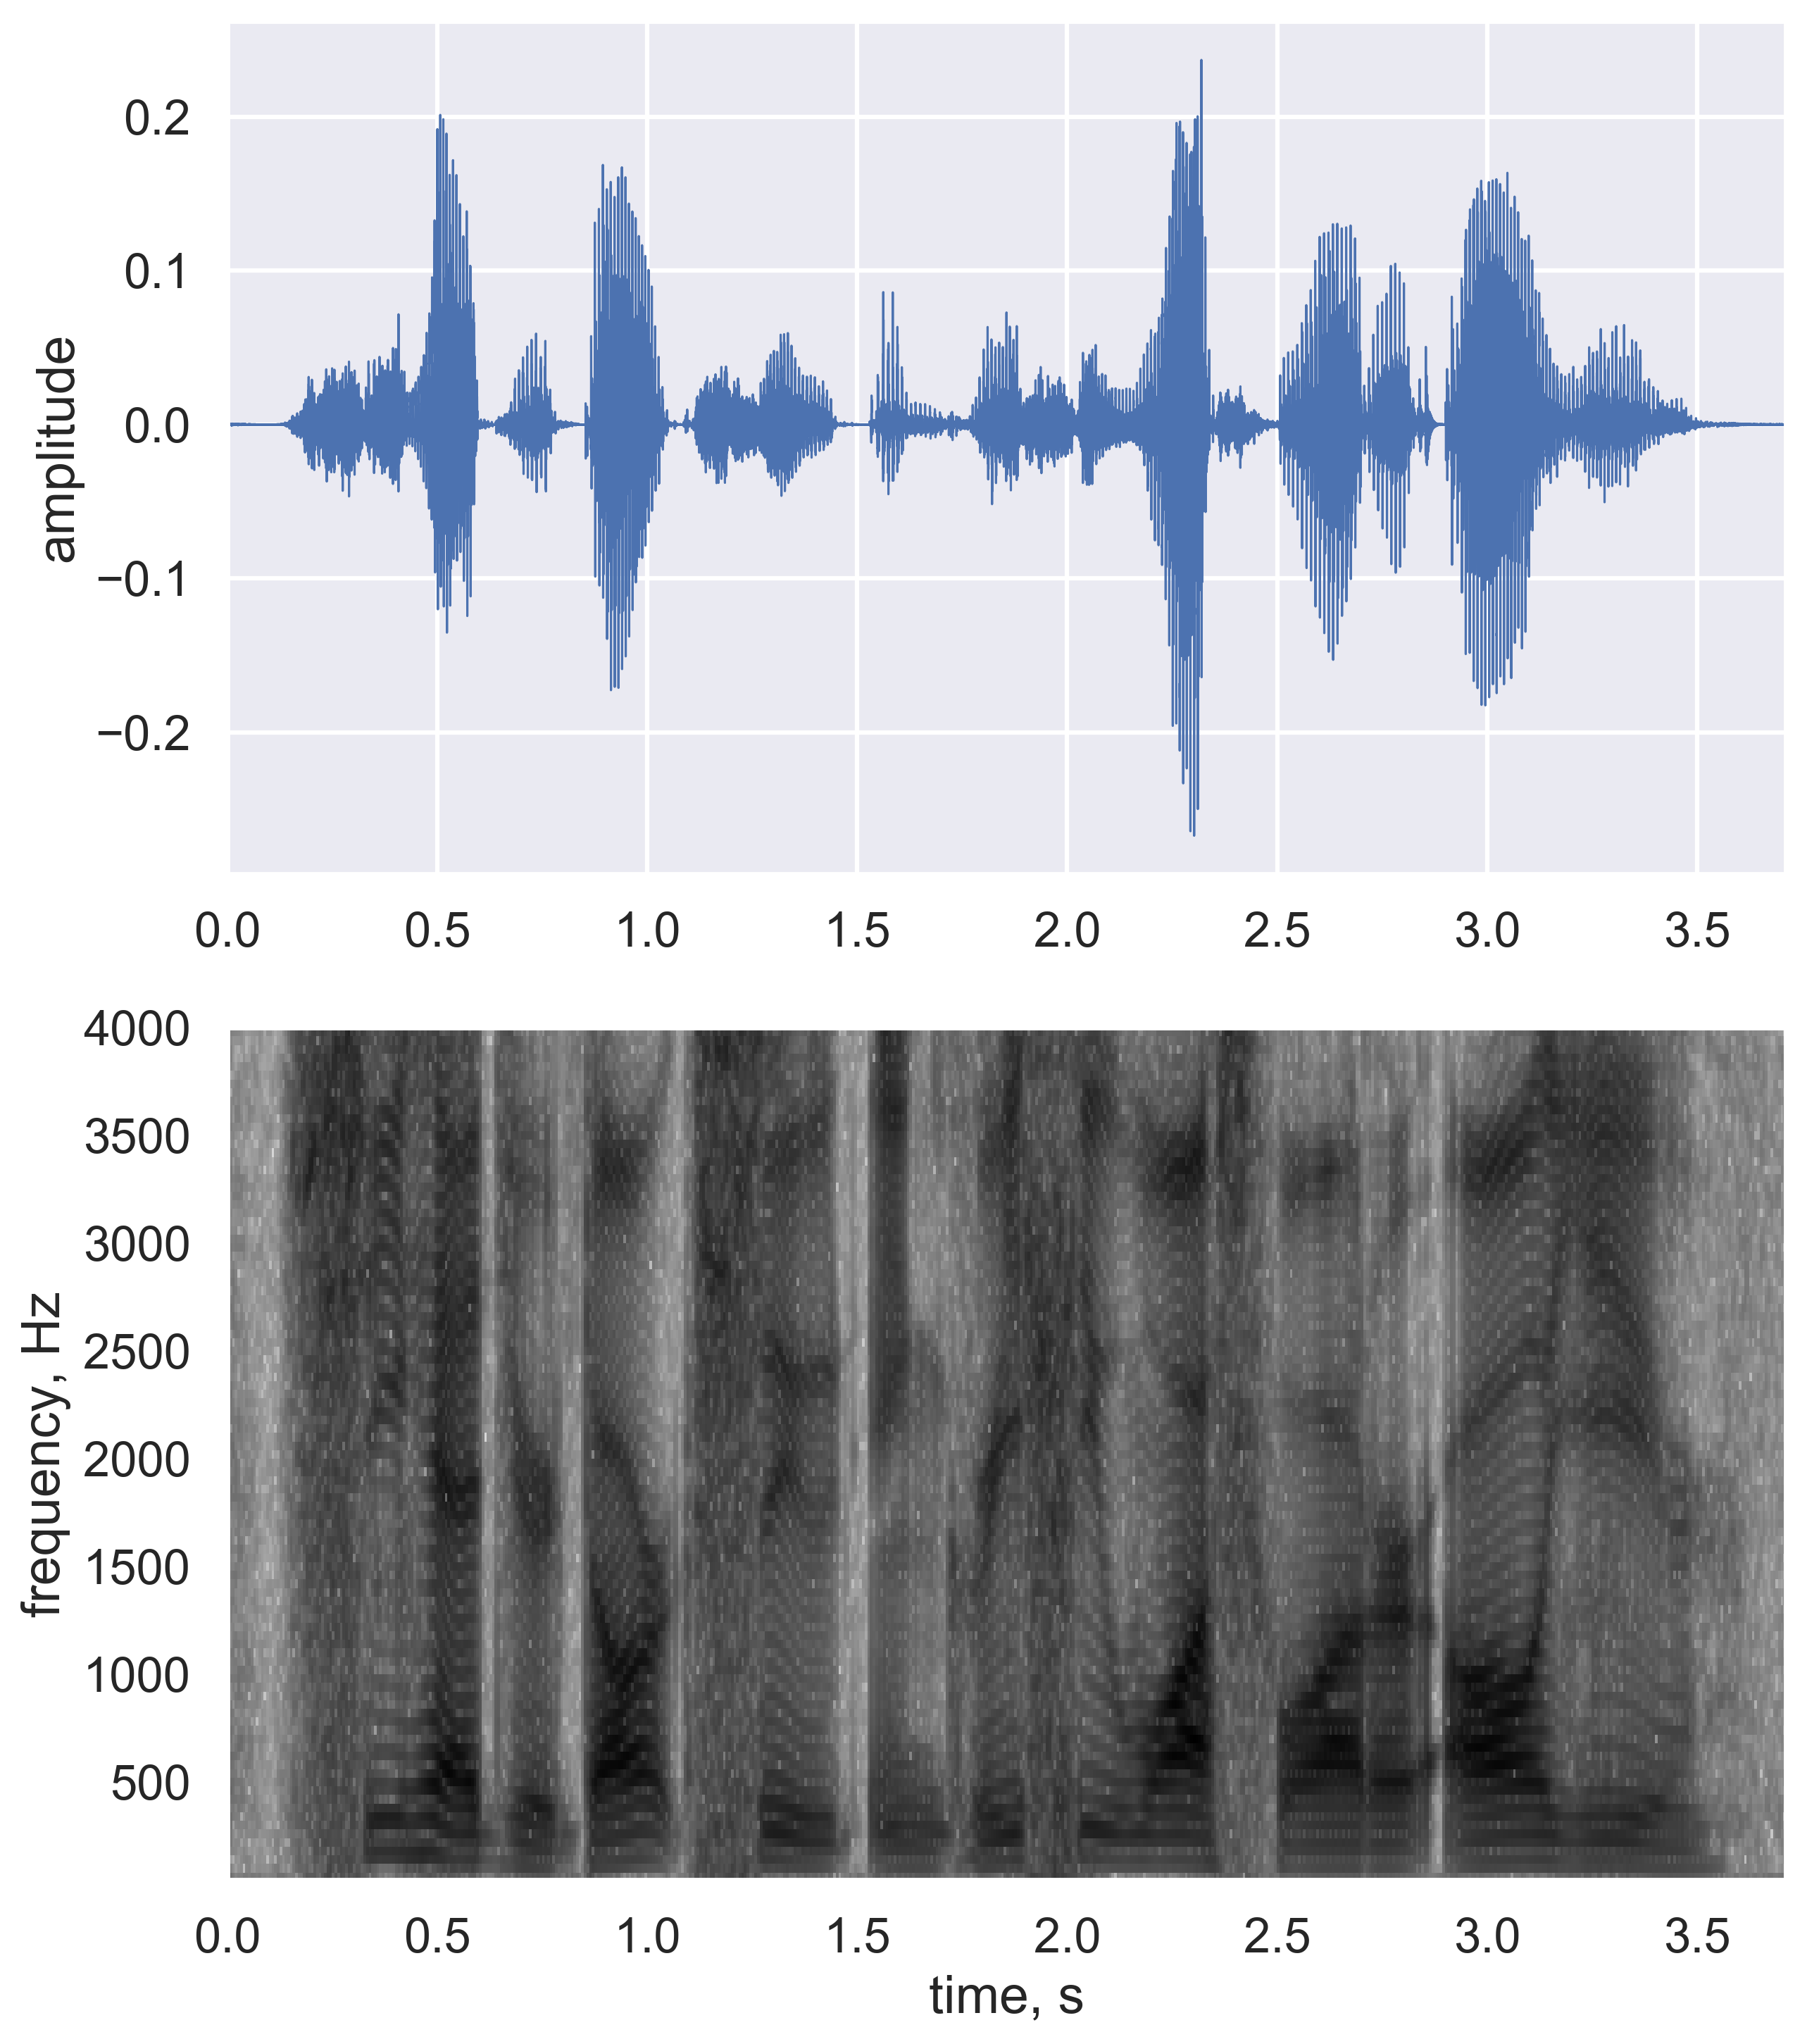
\includegraphics[width=0.46\textwidth]{original.png}\label{fig:original}}}}
	\quad % or other spacing between figures
	\subfloat[Recovered]{\makebox[0.46\textwidth]{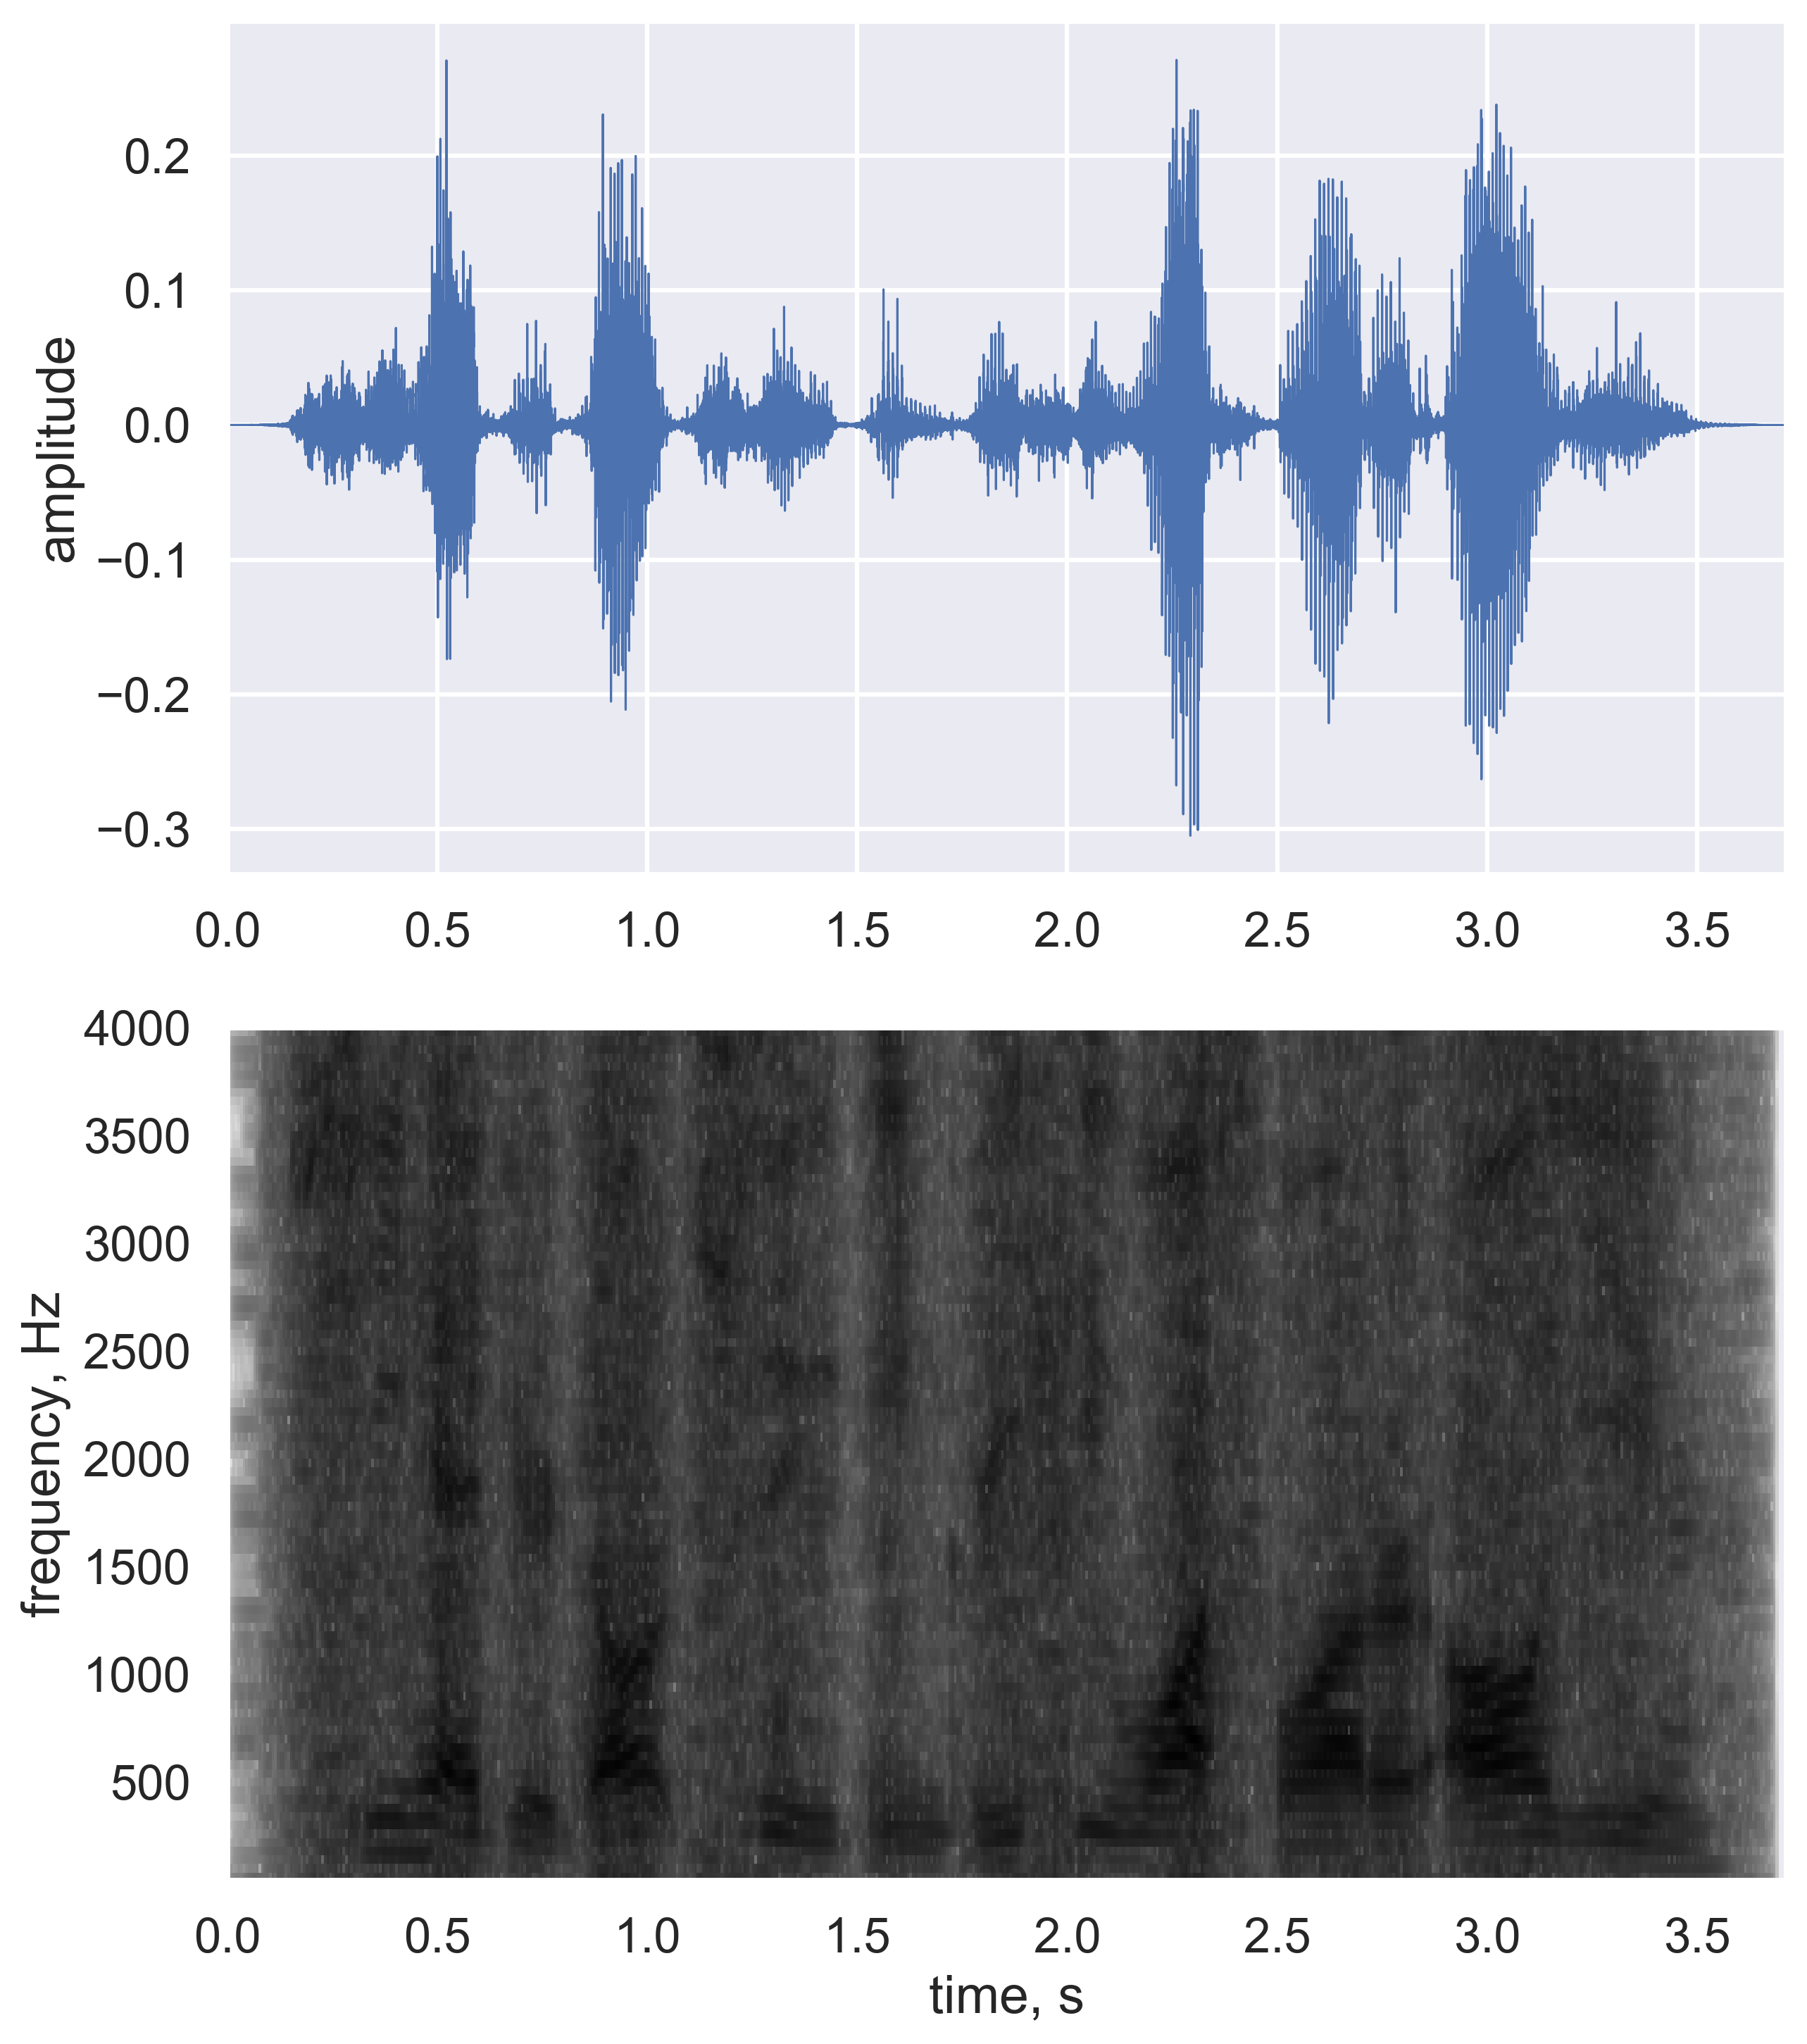
\includegraphics[width=0.46\textwidth]{recovered.png}\label{fig:recovered}}}
	\caption{Test speech signal obtained from the TIMIT speech corpus with the (a) original signal, and (b) reconstructed signal from compressive measurements. The top row is the representation in the time domain, while the bottom row is the spectrogram representation (25 ms sampling window with 75\% overlap). The signal reads ``She had your dark suit in greasy wash water all year''.}\label{fig:spectrogram}
\end{figure}

\begin{figure}[tb]
	\centering
	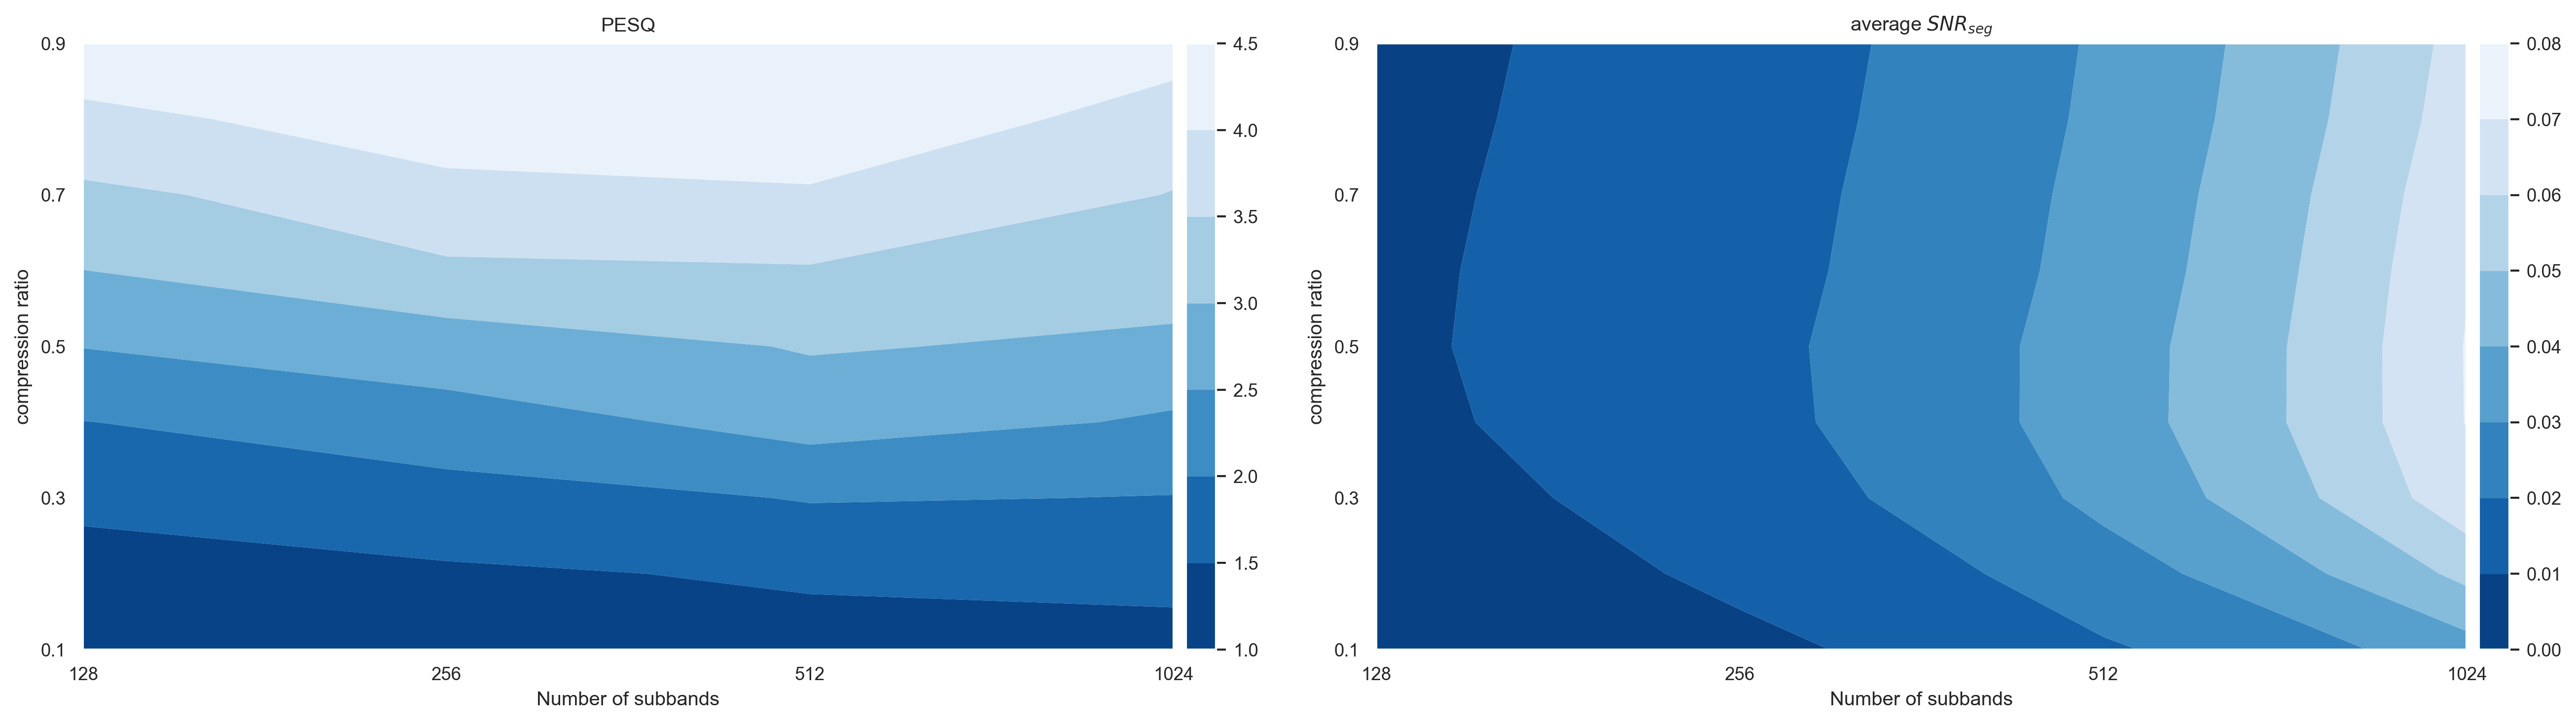
\includegraphics[width=\textwidth]{metrics.png}
	\caption{Two most commonly used metrics in evaluating quality of reconstructed speech recordings. PESQ is sensitive to the signal compression (left), while the \snrseg~is sensitive to the number of subbands (right).}
	\label{fig:pesq-snr}
\end{figure}


\section{Conclusions}
Here is the Summary or Conclusions section.


\bibliographystyle{spp-bst}
\bibliography{bibfile}

\end{document}